\section{Octree}

Ein Octree ist zunächst eine Datenstruktur, die wie ein Baum mit beliebiger Tiefe aufgebaut ist und pro Knoten Acht Kinder besitzt. Die Funktion ist dabei in \(\mathbb{R}^3\) gleich zu einem Binärbaum in \(\mathbb{R}\) oder einem Quadtree in \(\mathbb{R}^2\). Ein Knoten repräsentiert im Octree einen Würfel, der durch seine Kinder in Acht Kind-Würfel aufgeteilt wird. Diese Aufteilung ist in Abbildung \ref{fig:octree} exemplarisch dargestellt.\\

\begin{figure}[h]
  \centering
	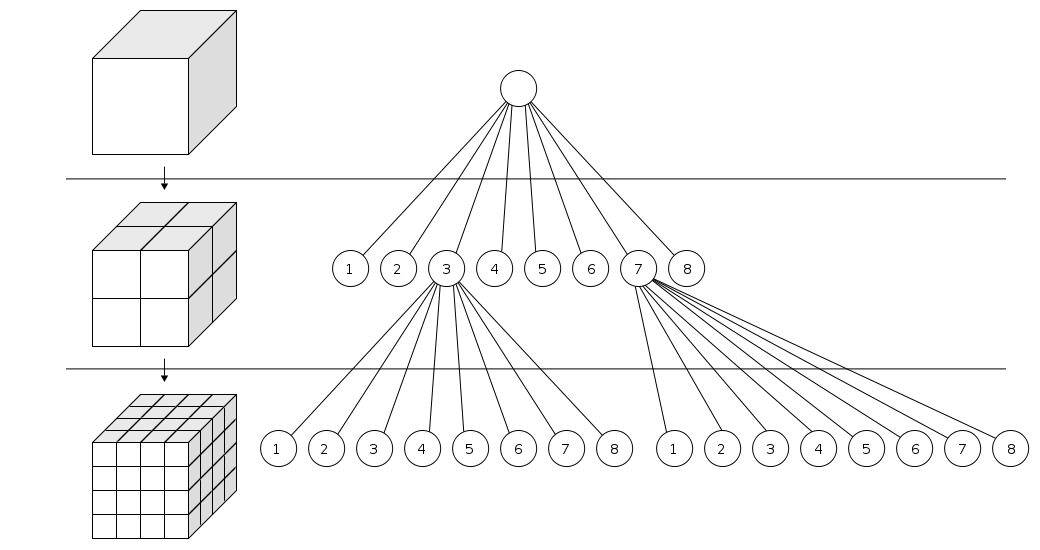
\includegraphics[width=1.0\textwidth]{content/images/theory/octree.png} 
  \caption{Schematische Darstellung eines Octrees mit zwei Untergliederungen. Übernommen von \citet{dumusc2011multi}}
  \label{fig:octree}
\end{figure}

Durch diese räumliche Aufteilung ergeben sich verschiedene Vorteile gegenüber linearen Datenstrukturen. So müssen Bereiche zum festhalten räumlicher Informationen im Octree nur dann allokiert werden, wenn diese Bereiche auch verwendet werden. Außerdem kann man mit Hilfe von Octrees ein einfaches Downsampling von Daten ermöglichen. Speichert man Punkte in den untersten Knoten eines Octrees kann man durch eine Tiefenbegrenzung beim Zugriff auf den Baum ein sehr effektives Downsampling der Punkte vornehmen. Zudem kann ein Octree zum einfachen räumlichen Clustern von dreidimensionalen Objekten dienen.\\